\documentclass[a4paper, 11pt, titlepage]{article}
\usepackage[utf8]{inputenc}
\usepackage[czech]{babel}
\usepackage[total={18.5cm,25cm}, top=3cm, left=1.25cm, includefoot]{geometry}
\usepackage{fancyhdr}
\usepackage{amsmath} % větší zlomyk pmocí \dfrac
\usepackage{graphicx}
\usepackage{float} % H aby neuplavali
\usepackage{ctable} % horozontální čára s nastavitelnou šířkou a mezerami od okolí \specialrule{1pt}{0pt}{0pt} 
\usepackage{array}
\usepackage{caption}
\usepackage{subcaption}

\newcommand{\nazevprace}{PROTOKOL O MĚŘENÍ}
\newcommand{\uloha}{OSCILÁTOR S WIENOVÝM ČLÁNKEM}
\newcommand{\pcislo}{201-4R} 			% číslo protokolu

\newcommand{\trida}{4A}
\newcommand{\skupina}{3}
\newcommand{\jmeno}{Jan}
\newcommand{\prijmeni}{VYKYDAL}
\newcommand{\porc}{26}						% pořadové číslo v třídní knize

\newcommand{\rok}{2014/2015}
\newcommand{\datm}{11.3.} 				% datum měření
\newcommand{\dato}{23.4.} 				% datum odevzdání


\pagestyle{fancy}
\fancyhf{}

\fancyfoot[C]{
  \begin{tabular}[H]{|c|c|c|c|}
    \hline
    \textbf{Jméno PŘÍJMENÍ:} \jmeno~\prijmeni & \textbf{Třída:} \trida & \textbf{Číslo protokolu:} \pcislo & \textbf{List:} \thepage/\pageref{konec} \\
    \hline
  \end{tabular}
}

\renewcommand{\headrulewidth}{0.0pt}
%\renewcommand{\footrulewidth}{0.4pt}


\begin{document} 
	
	
	\renewcommand{\figurename}{Schéma č.}
	\renewcommand{\tablename}{Tabulka č.}
	
  \begin{titlepage}
  \renewcommand{\arraystretch}{1.3}
  \pagestyle{empty}
  \begin{center}
    \begin{tabularx}{\textwidth}{!{\vrule width 2pt}XX!{\vrule width 1pt}XX!{\vrule width 1pt}XX!{\vrule width 1pt}X!{\vrule width 1pt}X!{\vrule width 1pt}X!{\vrule width 1pt}X!{\vrule width 2pt}}
      \specialrule{2pt}{0pt}{0pt}
      %\multicolumn{10}{!{\vrule width 2pt}c!{\vrule width 2pt}}{} \\
      \multicolumn{10}{!{\vrule width 2pt}c!{\vrule width 2pt}}{\Large Vyšší odborná škola a Střední průmyslová škola elektrotechnická} \\
      %\multicolumn{10}{!{\vrule width 2pt}c!{\vrule width 2pt}}{} \\
      \multicolumn{10}{!{\vrule width 2pt}c!{\vrule width 2pt}}{\Large Božetěchova 3, Olomouc} \\
      %\multicolumn{10}{!{\vrule width 2pt}c!{\vrule width 2pt}}{} \\
      \multicolumn{10}{!{\vrule width 2pt}c!{\vrule width 2pt}}{\Large Laboratoře elektronických měření} \\
      %\multicolumn{10}{!{\vrule width 2pt}c!{\vrule width 2pt}}{} \\
      \specialrule{1pt}{0pt}{0pt} 
      \multicolumn{10}{!{\vrule width 2pt}c!{\vrule width 2pt}}{} \\
      \multicolumn{10}{!{\vrule width 2pt}c!{\vrule width 2pt}}{\bf\Huge PROTOKOL O MĚŘENÍ} \\
      \multicolumn{10}{!{\vrule width 2pt}c!{\vrule width 2pt}}{} \\
      \specialrule{1pt}{0pt}{0pt}
      
      
      \multicolumn{8}{!{\vrule width 2pt}l!{\vrule width 1pt}}{Název úlohy} &
      \multicolumn{2}{l!{\vrule width 2pt}}{Číslo úlohy} \\
      \multicolumn{8}{!{\vrule width 2pt}c!{\vrule width 1pt}}{\Large\bf GENERÁTOR S IO555} &
      \multicolumn{2}{c!{\vrule width 2pt}}{\Large\bf 101-3R} \\
      \specialrule{1pt}{0pt}{0pt} 
      
      \multicolumn{1}{!{\vrule width 2pt}l}{Zadání} &
      \multicolumn{9}{l!{\vrule width 2pt}}{} \\
      \multicolumn{1}{!{\vrule width 2pt}l}{} &
      \multicolumn{9}{X!{\vrule width 2pt}}{\begin{minipage}[H][11.48cm][c]{0.8\textwidth}
	\begin{enumerate}
		\item
			Navrhněte oscilátor s Wienovým článkem RC, operačním zesilovačem MA 741CN a žárovkovou stabilizací napětí, požadován rozsah frekvencí $f_{min} = 300~Hz$ až $f_{max} = 7~kHz$. Napájecí napětí volte $\pm 15~V$, $C_1 = C_2 = 220~nF$.
		\item
			Sestavte navržený oscilátor, nastavte jeho optimální režim a změřte:
			\begin{enumerate}
				\item        
					skutečný frekvenční rozsah, změřený s vypočítanými a zapojenými součástkami
				\item
					závislost velikosti výstupního napětí na frekvenci, v rozsahu fmin až fmax a sestrojte graf
			\end{enumerate}                
		\item
			Vypočítejte procentní chybu změny výstupního napětí oscilátoru při přelaďování frekvence a sestavte graf na PC.
		\item
			Změřte maximální frekvenci, při které ještě nedochází ke znatelné změně velikosti nebo tvaru výstupního napětí.     
	\end{enumerate}
\end{minipage}


} \\
      \specialrule{1pt}{0pt}{0pt} 
      
      \multicolumn{1}{!{\vrule width 2pt}l!{\vrule width 1pt}}{Poř. č.} &
      \multicolumn{5}{l!{\vrule width 1pt}}{PŘÍJMENÍ a Jméno} &
      \multicolumn{1}{c!{\vrule width 1pt}}{Třída} &
      \multicolumn{1}{c!{\vrule width 1pt}}{Skupina} &
      \multicolumn{2}{l!{\vrule width 2pt}}{Školní rok} \\
      \specialrule{1pt}{0pt}{0pt} 
      
      \multicolumn{1}{!{\vrule width 2pt}c!{\vrule width 1pt}}{\Large\bf 26} &
      \multicolumn{5}{c!{\vrule width 1pt}}{\Large\bf VYKYDAL Jan} &
      \multicolumn{1}{c!{\vrule width 1pt}}{\Large\bf 3A} &
      \multicolumn{1}{c!{\vrule width 1pt}}{\Large\bf 3} &
      \multicolumn{2}{c!{\vrule width 2pt}}{\Large\bf 2013/2014} \\
      \specialrule{1pt}{0pt}{0pt} 
      
      \multicolumn{2}{!{\vrule width 2pt}l!{\vrule width 1pt}}{Datum měření} &
      \multicolumn{2}{l!{\vrule width 1pt}}{Datum odevzdání} &
      \multicolumn{2}{l!{\vrule width 1pt}}{Počet listů} &
      \multicolumn{4}{c!{\vrule width 2pt}}{Klasifikace} \\   
          
      \multicolumn{2}{!{\vrule width 2pt}c!{\vrule width 1pt}}{} &
      \multicolumn{2}{c!{\vrule width 1pt}}{} &
      \multicolumn{2}{c!{\vrule width 1pt}}{} &
      
      \multicolumn{1}{c!{\vrule width 1pt}}{příprava} &     
      \multicolumn{1}{c!{\vrule width 1pt}}{meření} &     
      \multicolumn{1}{c!{\vrule width 1pt}}{protokol} &     
      \multicolumn{1}{c!{\vrule width 2pt}}{obhajoba} \\ 
      
      
      
      \multicolumn{2}{!{\vrule width 2pt}c!{\vrule width 1pt}}{\Large\bf 17.3.} &
      \multicolumn{2}{c!{\vrule width 1pt}}{\Large\bf 24.3.} &
      \multicolumn{2}{c!{\vrule width 1pt}}{\Large\bf \pageref{konec}} &
      \multicolumn{1}{c!{\vrule width 1pt}}{} &     
      \multicolumn{1}{c!{\vrule width 1pt}}{} &     
      \multicolumn{1}{c!{\vrule width 1pt}}{} &     
      \multicolumn{1}{c!{\vrule width 2pt}}{} \\     
      &&&&&&&&&\\
      \specialrule{1pt}{0pt}{0pt} 
       
      \multicolumn{10}{!{\vrule width 2pt}l!{\vrule width 2pt}}{Protokol o měření obsahuje:} \\
      \multicolumn{10}{!{\vrule width 2pt}X!{\vrule width 2pt}}{\hspace*{-3mm}
\begin{tabular}{lll}%\hspace*{-2.2mm}
  Protokol o měření obsahuje: & Teoretický úvod             & Tabulky naměřených a vypočtených hodnot \\
   & Schéma                      & Vzor výpočtu                            \\
   & Tabulka použitých přístrojů & Grafy                                   \\
   & Postup měření               & Závěr                                   \\
\end{tabular}
} \\
      \specialrule{2pt}{0pt}{0pt} 
    \end{tabularx}  
  \end{center}
\end{titlepage}

  \setcounter{page}{2}
  \section*{Teoretický úvod}
		\subsection*{Dolní propust}
			\indent\indent
			Dolní propust je dvojbran, který tlumí signály o frekvenci  vyšší než je mezní frekvence tohoto obvodu. Základní pasivní doplní propust se dá vytvořit se dvou pasivních součástek a to: RC, RL a LC. V našem případě byla použita varianta RC a tak si ji popíšeme. RC dolní propust může být tvořena jedním rezistorem a jedním kondenzátorem. Tyto prvky jsou zapojeny jako klasický dělič napětí (kondenzátor je dole a odebíráme z něj výstupní napětí). Tento dělič je frekvenčně závislí a to na aktuální kapacitní reaktanci použitého kondenzátoru. Toto zapojení se někdy také označuje jako integrační článek. Ale v našem případě by to bylo chybné označení, protože o integračním článku se bavíme tehdy, řešíme-li přechodové děje, nebo-li odezvu na jednotkový impulz.
			
			Vztah pro výpočet mezní frekvence dolní a zároveň také horní propusti:
			\begin{equation}
  				f_0 = \dfrac{1}{2\pi R C} \Rightarrow R = \dfrac{1}{2\pi f_0 C}
  			\end{equation}		
		
			\hspace*{2cm}kde:\newline    
  			\hspace*{4cm}$f_0$ \dotfill mezní frekvence\hspace*{4cm}\newline
	  		\hspace*{4cm}$R$ \dotfill rezistor\hspace*{4cm}\newline
	  		\hspace*{4cm}$C$ \dotfill kondenzátor\hspace*{4cm}\newline
			
		
		\subsection*{Horní propust}
			\indent\indent
			Jedná se o dvojbran, který potlačuje signály o kmitočtu nižším, nežli je mezní frekvence tohoto filtru. Jedná se o obdobu filtru popsaného výše, s tím rozdílem, že nahradíme pořadí použitých součástek a výstupní napětí budeme odebírat s rezistoru. Pro výpočet mezní frekvence platí stejný vztah, jako pro výpočet mezní frekvence dolní propusti.
		
		
		\subsection*{Neinvertující zesilovač s OZ}
			\indent\indent
			Neinvertující zesilovač s OZ je zapojení, které zesiluje vstupní signál a přitom neobrací fázi vstupního signálu. Jeho předností je velký vstupní odpor v řádů několika $M\Omega$. V našem případě je ale vstupní odpor snižován rezistorem dolní propusti.
			
			
			Vztah pro výpočet mezní frekvence použitého integračního článku:
			\begin{equation}
  				a_u = 20\log\frac{R_{2}}{R_1} + 1 \Rightarrow R_{2} = R_1 (10^{\frac{a_u}{20}} - 1)
  			\end{equation}		
		
			\hspace*{2cm}kde:\newline    
  			\hspace*{4cm}$a_u$ \dotfill napěťový zisk\hspace*{4cm}\newline
	  		\hspace*{4cm}$R_1$ \dotfill rezistor\hspace*{4cm}\newline
	  		\hspace*{4cm}$R_{2}$ \dotfill rezistor\hspace*{4cm}\newline
  				

  
		\subsection*{Napěťový sledovač s OZ}
			\indent\indent
			Jedná se o takové zapojení OZ, kdy vstupní signál je přiváděn na neinvertující vstup OZ a výstupní signál tvoří zápornou napěťovou zpětnou vazbu. Napěťový sledovač se tomuto obvodu říká proto, že výstupní napětí sleduje napětí vstupní. Jinými slovy $U_{OUT} = U_{IN}$. Protože zpětná vazba nám odečte zesílení obvodu. Tento obvod se nejčastěji používá pro oddělování různých obvodů od sebe. Slouží jako impedanční transformace. Na vstupu má obvod velký vstupní odpor v řádu několika $M\Omega$. Výstupní odpor je zpravidla nízký a pohybuje se v řádu desítek $\Omega$.


  \clearpage
  \section*{Schémata}
  \begin{figure}[H]
    \centering
    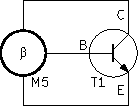
\includegraphics[width=4cm]{../img/BETA.pdf}
    \caption{Orientační měření $\beta$}
    \label{sch:2}
  \end{figure}
  
  \begin{figure}[H]
    \centering
    
\includegraphics[width=18cm]{../img/SCH1.pdf}
    \caption{Měření napěťového přenosu a frekvenčních charakteristik}
    \label{sch:2}
  \end{figure}
  
  \begin{figure}[H]
    \centering
    
\includegraphics[width=16cm]{../img/SCH2.pdf}
    \caption{Měření vstupního odporu (část 1.)}
    \label{sch:2}
  \end{figure}
  
  \begin{figure}[H]
    \centering
    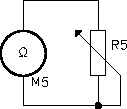
\includegraphics[width=4cm]{../img/OHM.pdf}
    \caption{Měření hodnoty vstupního odporu (část 2.)}
    \label{sch:2}
  \end{figure}


  \section{Tabulka použitých přístrojů}
  \begin{table}[H]
    \begin{center}
      \begin{tabular}[H]{!{\vrule width 1pt}c|c|c|c|c!{\vrule width 1pt}}
      \specialrule{1pt}{0pt}{0pt} 
      \textbf{Označení v zapojení} & \textbf{Přístroj} & \textbf{Typ} & \textbf{Evidenční číslo} &\textbf{Poznámka} \\\specialrule{1pt}{0pt}{0pt} 
      
      $-$   & DMM           & MASTECH MY-64     & $0659$  & $-$ \\\hline
      $FG$  & generátor     & GoldStar FG-2002C & $0382$  & $-$ \\\hline
      $mV$  & milivoltmetr  & TESLA BK-128      & $0132$  & $-$ \\\specialrule{1pt}{0pt}{0pt} 
          
    \end{tabular}
      
      \caption{Tabulka použitých přístrojů}
      \label{tab:metr}      
    \end{center}
  \end{table}

  \section*{Postup měření}
  \subsection*{Zapojení obvodu}
    \begin{itemize}
      \item
      	Ze zadaných parametrů dopočítáme požadované hodnoty součástek.
      \item
      	Součástky, které jsme vypočítali připojíme k měřícímu přípravku.
      \item
        K obvodu připojíme měřící systém UNIMA a zdroj napětí. 	
	\end{itemize}

		
 

  \section{Tabulky naměřených a vypočítaných hodnot}
  
  \begin{table}[H]
    \begin{center}
      \begin{tabular}[H]{!{\vrule width 1pt}c|c|c|c|c|c!{\vrule width 1pt}}
        \specialrule{1pt}{0pt}{0pt} 
        \textbf{$R_2~[k\Omega]$} & \textbf{$U_{OUT}~[V]$} & \textbf{$\%_{chyba}~[\%]$} & \textbf{$\Delta_{chyba}~[mV]$} & \textbf{$U_{OUT_{VYP}}[V]$} & \textbf{$\Delta{U_{OUT_{VYP}}-U_{OUT}}~[V]$} \\\specialrule{1pt}{0pt}{0pt} 
        $5$ & $-0,81$ & $1,73$ & $14,00$ & $-0,8$ & $0,01$\\\hline
        $10$ & $-1,62$ & $1,11$ & $18,10$ & $-1,6$ & $0,02$\\\hline
        $20$ & $-3,23$ & $0,81$ & $26,15$ & $-3,2$ & $0,03$\\\hline
        $40$ & $-6,46$ & $0,65$ & $42,30$ & $-6,4$ & $0,06$\\\hline
        $60$ & $-9,68$ & $0,60$ & $58,40$ & $-9,6$ & $0,08$\\\hline
        $80$ & $-12,91$ & $0,58$ & $74,55$ & $-12,8$ & $0,11$\\\hline
        $100$ & $-13,30$ & $0,57$ & $76,50$ & $-16,0$ & $2,70$
        \\\specialrule{1pt}{0pt}{0pt} 
        
      \end{tabular}
      
      \caption{Měření $U_{OUT} = f(R_2)$ zapojení dle schématu č. 4}
      \label{tab:s1}      
    \end{center}
  \end{table}
  
  \begin{table}[H]
    \begin{center}
      \begin{tabular}[H]{!{\vrule width 1pt}c|c|c|c!{\vrule width 1pt}}
        \specialrule{1pt}{0pt}{0pt} 
        \textbf{$R_1~[k\Omega]$} & \textbf{$U_{OUT}~[V]$} & \textbf{$\%_{chyba}~[\%]$} & \textbf{$\Delta_{chyba}~[mV]$}\\\specialrule{1pt}{0pt}{0pt} 
        $5$ & $1,496$ & $0,86$ & $12,866$ \\\hline
        $10$ & $0,750$ & $0,83$ & $6,255$ \\\hline
        $20$ & $0,373$ & $0,82$ & $3,048$ \\\hline        
        $40$ & $199,2\cdot 10^{-3}$ & $0,81$ & $1,609$ \\\hline
        $60$ & $134,7\cdot 10^{-3}$ & $0,81$ & $1,0843$ \\\hline
        $80$ & $99,6\cdot 10^{-3}$ & $0,80$ & $0,800$ \\\hline
        $100$ & $79,7\cdot 10^{-3}$ & $0,80$ & $0,634$ 
        \\\specialrule{1pt}{0pt}{0pt} 
        
      \end{tabular}
      
      \caption{Měření $U_{OUT} = f(R_1)$ zapojení dle schématu č. 5}
      \label{tab:s1}      
    \end{center}
  \end{table}
  

  \section*{Vzory výpočtů}
  
  Výpočet geometrického průměru kondenzátoru $C$:
  \begin{equation}
    C = \sqrt{C_1 \cdot C_2} = \sqrt{34,16 \cdot 32,1} \doteq \underline{\underline{33,09~nF}}
    \nonumber
  \end{equation}
  
  Výpočet odporu rezistoru $R_1$ a $R_2$ provádíme dosazením do upraveného vztahu (1) pro dolní frekvenci 
  \begin{equation}
    R = \dfrac{1}{2\pi f_0 C} = \dfrac{1}{2\pi \cdot 300 \cdot 33,09 \cdot 10^{-9}} \doteq \underline{\underline{16~k\Omega}}
    \nonumber
  \end{equation}   
  
  Výpočet odporu rezistoru $R_1$ a $R_2$ provádíme dosazením do upraveného vztahu (1) pro horní frekvenci 
  \begin{equation}
    R = \dfrac{1}{2\pi f_0 C} = \dfrac{1}{2\pi \cdot 7000 \cdot 33,09 \cdot 10^{-9}} \doteq \underline{\underline{689~\Omega}}
    \nonumber
  \end{equation}     
  
  Střední hodnota výstupního napětí $U_{OUT_{AV}}$:
  \begin{equation}
    U_{OUT_{AV}} = \dfrac{U_{OUT_{MAX}} - U_{OUT_{MIN}}}{2} = \dfrac{7,4 - 7,3}{2}  \underline{\underline{7,35~V}}
    \nonumber
  \end{equation} 
    
  Výpočet procentní chyba výstupního napětí:
  \begin{equation}
    \delta_f = \dfrac{U_{OUT_{MAX}} - U_{OUT_MIN}}{U_{OUT_{AV}}} \cdot 100 = \dfrac{7,4 - 7,3}{7,35} \cdot 100 \doteq \underline{\underline{1,36~\%}}
  	\nonumber
  \end{equation}
  
  \section*{Grafy}
\setcounter{figure}{0}
\renewcommand{\figurename}{Graf č.}
  
  \begin{figure}[H]
    \centering
    \includegraphics[width=14cm]{../img/g1.png}
    \caption{Velikost výstupního napětí.($0,5~\frac{V}{d}$ a $5~\frac{\mu s}{d}$) }
    \label{gra:1}
  \end{figure}
  
  \begin{figure}[H]
    \centering
    \includegraphics[width=16cm]{../img/g2.png}
    \caption{frekvenční přenosová charakteristika zesilovače s OZ a horní propustí $a_U = f(f)$}
    \label{gra:1}
  \end{figure}
  
  \begin{figure}[H]
    \centering
    \includegraphics[width=16cm]{../img/g3.png}
    \caption{frekvenční přenosová charakteristika zesilovače s OZ, horní a dolní propustí a sledovačem $a_U = f(f)$}
    \label{gra:1}
  \end{figure}    

 
   
  \section{Závěr}
  \subsection{Chyby měřících přístrojů}
    \indent\indent
    Procentuální chyba milovoltmetru se pobybovala v intervalu $<\pm 3~\%;~\pm 5~\%>$. Tento měřící přístoj tety nespadá do kategorie těch nejpěsnější, nicměně lepší přístoj pro malá napětí  o vysokých frekvencích jsme neměli k dospozici.
  
  \subsection{Zhodnocení}
    \begin{enumerate}
      \item
        V úvodu jsem shrnul základní poznatky o paralerním a sériovém rezonačním obvodu, takže bych měl mít bod 1 splněný.
      \item
        Změřil jsem frekvenční charakteristiku sériového rezonančního obvodu v rozsahu $\pm 50~kHz$ kolem rezonanční frekvence $f_0$. Naměřené charakteristika není plně kompatibilní s teoretickým modelem tohoto zapojení. To může být způsobeno chybou měření nebo porazitními vlastnostmi použitého přípravku.
      \item
        Odpor $R_L$ byl spočítán s využitím vztahu (3). Jeho hodnota byla výpočtem určena na $196,9~\Omega$. Tata hodnota všek nemůže být povačována za správnou, protože jsem musel odvodit vztah ve kterém se nebude vyskytovat $C$. To bylo prakticky i teoreticky nemožné, tak sem jeho hodnotu $X_C$ zanedbal v doufání, že bude mít kapacitu větčí než $1~\mu F$. Z této vypočítané hodnoty jsem pak s využitém odpozeného vztahu (4) určil teoretickou inukčnost cívky $L$. Tu jsem stanovil na $196,6~\mu H$.
      \item
        Tento bod nebyl realizovatelný, protože nám nebyla sdělen jmenovité hodnota kondenzátoru~$C$. 
      \item
        Změřil jsem frekvenční charakteristiku paralerního rezonančního obvodu v rozsahu $\pm 50~kHz$ kolem rezonanční frekvence $f_0$. Naměřená charakteristika také není plně kompatibilní s teoretickým modelem tohoto zapojení.
      \item
        Změřil jsem frekvenční charakteristiku paralerního rezonančního obvodu se sníženým činitelem jakosti v rozsahu $\pm 50~kHz$ kolem rezonanční frekvence $f_0$. Naměřené charakteristika opět není plně kompatibilní s teoretickým modelem tohoto zapojení.
      \item
        Z naměřených hodnot jsem vytvořil grafy, ve vektorovém formátu *.eps, což se dá ocenit zejména při elektronickém prohlížení dokumentu.
    \end{enumerate}


  \label{konec}
\end{document}
